\documentclass{standalone}
\usepackage{tikz}
\usepackage{fourier}
\usetikzlibrary{mindmap,backgrounds}


\begin{document}


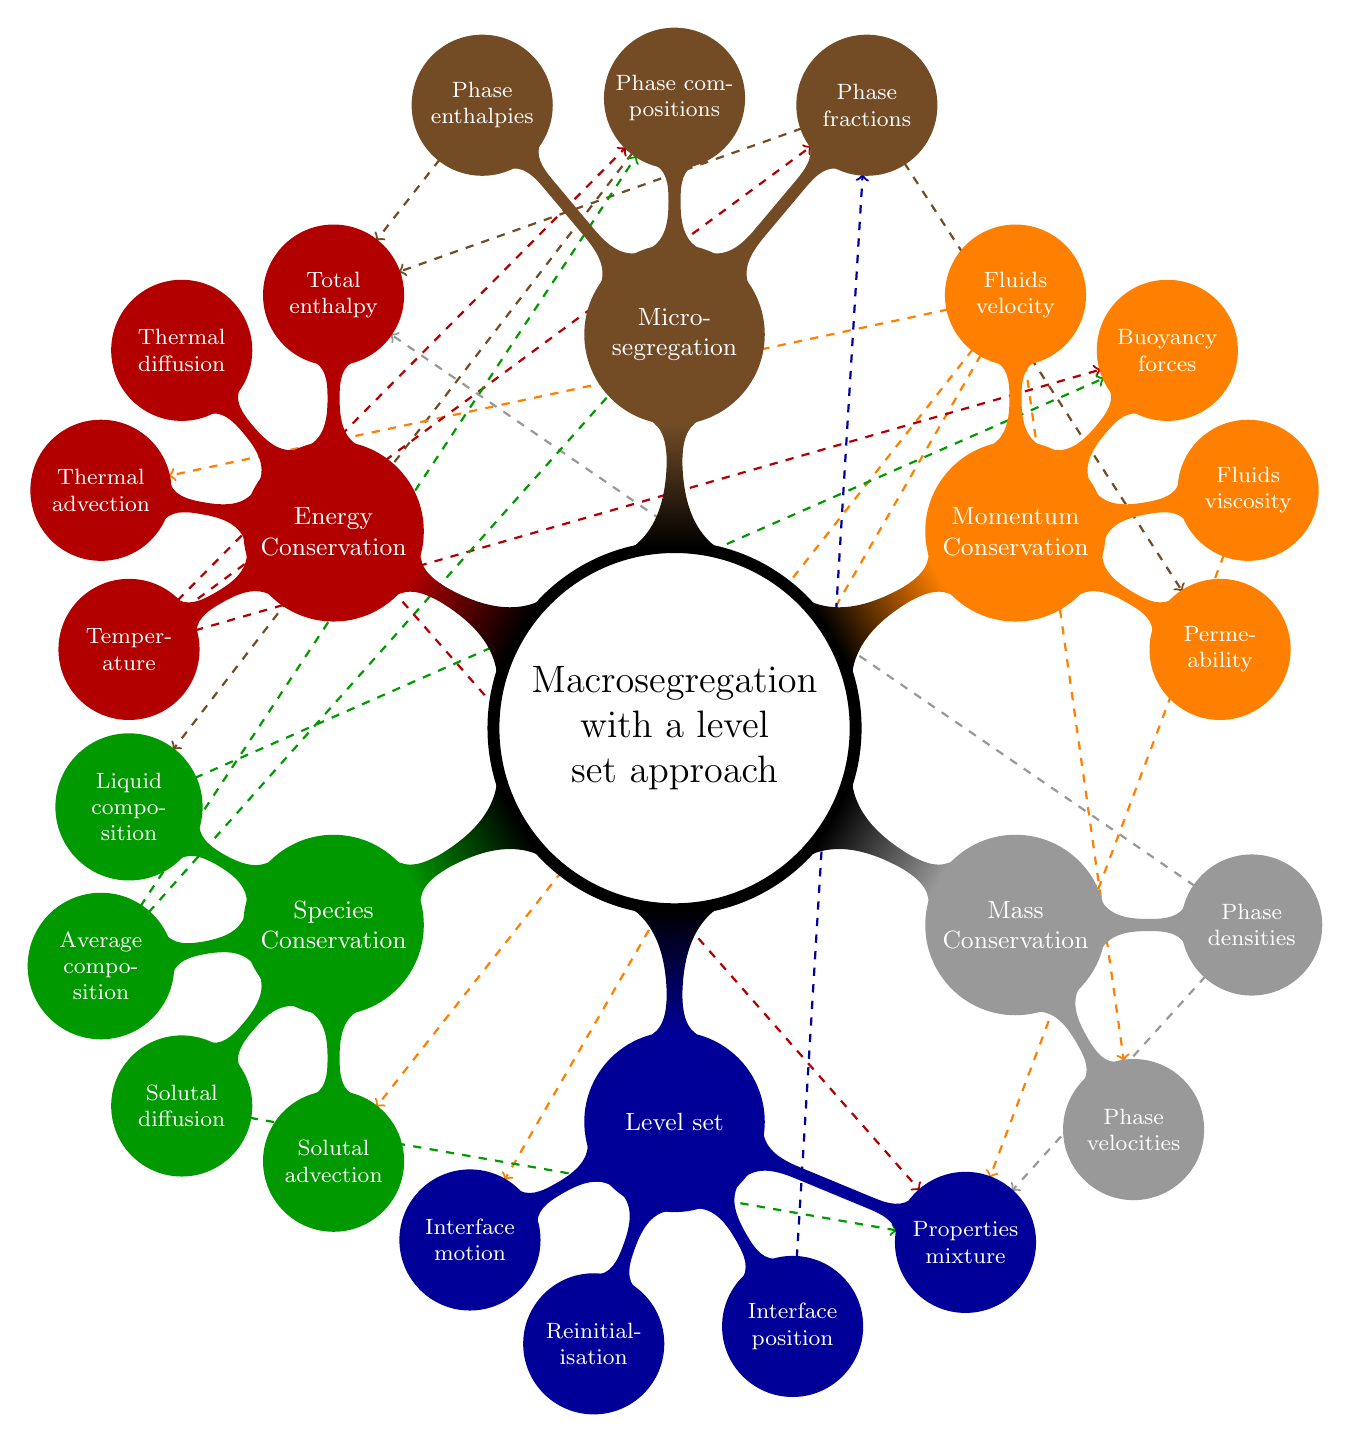
\begin{tikzpicture}[
  mindmap,
  every node/.style={concept, execute at begin node=\hskip0pt},
  root concept/.append style={
    concept color=black, fill=white, line width=1ex, text=black,
    scale=1.15
  },
  text=white, grow cyclic,  % cyclic % left %
  level 1/.append style={level distance=5cm,sibling angle=60},
  level 2/.append style={level distance=3cm,sibling angle=40},
]
%-------------------------------------------------------------
\newcommand{\coloris}{white!60!black}
\newcommand{\colorisE}{red!70!black}
\newcommand{\colorisM}{orange}
\newcommand{\colorisV}{white!60!black}
\newcommand{\colorisS}{green!60!black}
\newcommand{\coloriss}{brown!60!black}
\newcommand{\colorisL}{blue!60!black} 


\node[root concept] {Macrosegregation with a level set approach} % root
%============================================================
child[concept color=\colorisS] { node {Species Conservation}
child { node (S1) {Liquid composition}  } 
child { node (S2) {Average composition}  } 
child { node (S3) {Solutal diffusion} }
child { node (S4) {Solutal advection} }
}
%============================================================
child[concept color=\colorisL] { node  {Level set}
child { node (L1) {Interface motion} }
child  { node (L3) {Reinitialisation} }
child [sibling angle=60] { node (L2) {Interface position} }
child [sibling angle=45, level distance=4cm] { node (L4) {Properties mixture} }
}
%============================================================
child[concept color=\colorisV] { node {Mass Conservation}
child [sibling angle=60] { node (V1) {Phase velocities}  } 
child [sibling angle=60] { node (V2) {Phase densities}  }
}
%============================================================
child[concept color=\colorisM] { node  {Momentum Conservation}
child { node (M1) {Permeability}  } 
child { node (M2) {Fluids viscosity}  }
child { node (M3) {Buoyancy forces}  }
child { node (M4) {Fluids velocity}  }
}
%============================================================
child[concept color=\coloriss] { node  {Micro-segregation}
child [level distance=3.8cm] { node (s1) {Phase fractions} }
child { node (s2) {Phase compositions} }
child [level distance=3.8cm] { node (s3) {Phase enthalpies} }
}
%============================================================
child[concept color=\colorisE] { node  {Energy Conservation}
child { node (E1) {Total enthalpy}  } 
child { node (E3) {Thermal diffusion}  } 
child { node (E4) {Thermal advection} }
child { node (E2) {Temperature}  } 
};
%============================================================


\begin{pgfonlayer}{background}
	\draw[\coloriss, thick, dashed] (s1) edge[->] (M1);
	\draw[\coloriss, thick, dashed] (s2) edge[->] (S1);
	
	\draw[\coloriss, thick, dashed] (s3) edge[->] (E1);
	\draw[\colorisV, thick, dashed] (V2) edge[->] (E1);	
	\draw[\coloriss, thick, dashed] (s1) edge[->] (E1);

	\draw[\colorisM, thick, dashed] (M4) edge[->] (V1);
	\draw[\colorisM, thick, dashed] (M4) edge[->] (S4);
	\draw[\colorisM, thick, dashed] (M4) edge[->] (E4);
	\draw[\colorisM, thick, dashed] (M4) edge[->] (L1);
	
	\draw[\colorisE, thick, dashed] (E2) edge[->] (M3);
	\draw[\colorisS, thick, dashed] (S1) edge[->] (M3);
	
	\draw[\colorisE, thick, dashed] (E2) edge[->] (s1);
	\draw[\colorisE, thick, dashed] (E2) edge[->] (s2);
	\draw[\colorisS, thick, dashed] (S2) edge[->] (s1);
	\draw[\colorisS, thick, dashed] (S2) edge[->] (s2);
	
	\draw[\colorisL, thick, dashed] (L2) edge[->] (s1);
	
	\draw[\colorisS, thick, dashed] (S3) edge[->] (L4);
	\draw[\colorisV, thick, dashed] (V2) edge[->] (L4);
	\draw[\colorisM, thick, dashed] (M2) edge[->] (L4);
	\draw[\colorisE, thick, dashed] (E3) edge[->] (L4);

\end{pgfonlayer}

\end{tikzpicture}

\end{document}